\documentclass[12pt]{article} 
\usepackage[utf8]{inputenc}
\usepackage[T1]{fontenc}
\usepackage[french]{babel}
\usepackage{geometry} 
\geometry{a4paper} 

\usepackage{graphicx} 

\usepackage{float} 
\usepackage{wrapfig}

\linespread{1.2}

\setlength\parindent{2.5pt}

\graphicspath{{Pictures/}} 


\begin{document}
\begin{titlepage}
\newcommand{\HRule}{\rule{\linewidth}{0.5mm}}
\center 

\textsc{\LARGE Universtité de Lorraine}\\[1.5cm] 
\textsc{\Large Projet Tutoré}\\[0.5cm]
\textsc{\large ASRALL}\\[0.5cm]

\HRule \\[0.4cm]
{ \huge \bfseries Systèmes de Fichiers Distribués}\\[0.4cm] 
\HRule \\[1.5cm]

\begin{minipage}{0.4\textwidth}
\begin{flushleft} \large
\emph{Author:}\\
Ricardo \textsc{RODRÍGUEZ}\\
Julien \textsc{SCHNEIDER}\\
Jean \textsc{LUTZ}\\
Yannick \textsc{LAPREVOTTE}\\
\end{flushleft}
\end{minipage}
~
\begin{minipage}{0.4\textwidth}
\begin{flushright} \large
\emph{Supervisor:} \\
 Stephane \textsc{CASSET} 
\end{flushright}
\end{minipage}\\[4cm]

{\large \today}\\[3cm] 

\vfill 
\end{titlepage}


\tableofcontents 

\newpage 

\section{Introduction} 
\section{CEPH}
\newpage
\section{Lustre}

\begin{figure}[H] 
\center{
\includegraphics[width=0.5\linewidth]{placeholder}}
\caption{Lustre F.S.}
\label{fig:speciation}
\end{figure}

\subsection{Introduction}
Lustre est un système de fichiers distribué libre(sous licence GPL v2), utilisé pour de très grandes grappes de serveurs. Son nom vient de la combinaison de deux mots, «Linux» et «cluster». Le projet a commencé comme un projet de recherche en 1999 par Peter Braam, en 2007 Sun Microsystems a continué son développement, en 2010 avec l'acquisition de Sun, a commencé à manternir et sortir nouvelles versions de Lustre, en décembre du 2010 Oracle a arrêté le développement du système de fichiers version 2.x, plusieurs nouvelles organisations surgirent à fournir un soutien et de développement dans un modèle de développement communautaire ouvert, comprenant \textit{Whamcloud}, \textit{Open Scalable File Systes, Inc. (OpenSFS)}, \textit{EUROPEAN Open FileSystems (EOFS)} et autres. En 2012 WhamCloud a été rachetée par Intel.\\


Lustre a la possibilité de accueillir des dizaines de milliers de systèmes client et une grande quantité de données, pétaoctets\footnote{Un pétaoctet contient \begin{math}10^{15}\end{math} octets} de stockage et des centaines de gigaoctets(Go) de débit Entrée/Sortie. 

\subsubsection{Les composants de Lustre}
\begin{description}
\item[Serveur de Métadonnées \textit{(Metadata Server «MDS»)}:]
Le serveur MDS rend les métadonnées, stockées dans un ou plusieurs MDT, disponibles pour des clients Lustre. Chaque MDS gère les noms et répertoires dans le systèmes de fichiers Lustre.
\item[Cible de Métadonnées \textit{(Metadata Target «MDT»)}:] Le MDT stocke les métadonnées(tels que les noms de fichiers, les répertoires et la structure des fichiers) sur un MDS. Chaque système de fichiers possède un MDT. Une MDT sur une cible de stockage partagé peut être disponible pour de nombreux MDS, bien que l'on devrait utiliser effectivement. Si une MDS actif échoue, un MDS passif peut servir le MDT et le rendre disponible aux clients. Ceci est appelé \textit{MDS failover}.
\item[Serveur de Stockage d'Objets \textit{(Object Storage Server «OSS»)}:]
L'OSS fournit un servicce d'Entrée/Sortie de fichiers et \textit{network request handling} pour un ou plusieurs OST locaux. Typiquement, un OSS sert entre 2 et 8 OST, jusqu'à 8 To\footnote{Un téraoctet contient \begin{math}10^{12}\end{math}octets.}
\item[Cible de Stockage d'Objets \textit{(Object Storage Target «OST»)}:]
L'OST stocke les données(des morceaux de fichiers de l'utilisateur) comme des objets de données sur un ou plusieurs OSS. Un seul système de fichiers Lustre peut avoir plusieurs OST, servant chacun un sous-ensamble de fichiers données. Il n'est pas nécessairement une correspondance 1:1 entre un fichier et un OST. Pour optimiser les performances, un fichiers peut être distribué sur plusieurs OST.
\item[Serveur de Gestion \textit{(Management Server «MGS»)}:]
Le MGS stocke les informations de configuration pour tous les systèmes de fichiers Lustre dans une grappe de serveurs. Chaque component Lustre contacte le MGS pour fournir information, et les Lustre clients contactent le MGS pour obtenir information.
\item[Lustre clients:]Lustre clients sont noeuds éxecutant le logiciel Lustre qui leur permet de monter le système de fichiers Lustre.

Le logiciel client de Lustre est composé d'une interfacce entre le \textit{Linux Virtual File System} et les serveurs Lustre. Chaque cible(composant de Lustre) a une contrapartie client: Client de Métadonnées (MDC), Client de Stockage d'Objets(OSC) et un Client de Gestion(MGC). Un groupe de OSC sont intégrés dans un Volume d'objets logique(\textit{Logical Object Volume «LOV»}). Travaillant en collaboration, les OSC fournissent un accès transparent au système de fichiers.

Les clients qui montent le système de fichiers Lustre, voient un seul, cohérente, espace de noms(\textit{namespace}), synchronisé toujours. Différents clients peuvent écrire aux différentes parties d'un même fichier en même temps, tandis que d'autres clients peuvent lire le fichier.
\end{description}
\subsubsection{Principales Caractéristiques de Lustre}

Les principales caractéristiques de Lustre comprennent: \\

\begin{description}

\item[Évolutivité: ]
 Lustre échelles haut ou le bas par rapport au nombre de postes clients, stockage sur disque et bande passante. Actuellement , Lustre est en cours d'exécution dans des environnements de production avec un maximum de 26 000 postes clients, avec de nombreux grappes d'entre 10,000 et 20,000 clients. Autres installations fournissent Lustre d'espace de stockage en disque agrégé et bande passsante allant jusqu'à 1000 OST fonctionnant sur plus de 450 OSS. Plusieurs systèmes de fichiers Lustre avec une capacité de 1 pétaoctet ou plus (permettant le stockage de jusqu'à 2 milliards de fichiers) ont été en usage depuis 2006.
\item[Performance: ]
 Lustre déploiements dans des environnements de production offrent actuellement la performance de jusqu'à 100 Go par seconde. Dans un environnement de test, une performance de 130 Go par seconde a étée soutenue. Lustre seul débit de poste client a été mesurée à 2 Go par seconde (max) et OSS débit de 2,5 Go par seconde (max). Lustre a été exécuté à 240 Go par seconde sur le système de fichiers d'araignée(Spider File System) à Oak Ridge National Laboratories.

\item[Conformité POSIX:]Dans un cluster, la conformité POSIX signifie que la plupart des opérations sont atomiques et les clients ne voient jamais des données périmées ou métadonnées .
\item[Haute Disponibilité:]Lustre propose des partitions de stockage partagés pour les cibles de l'OSS (OST), et une partition de stockage partagé pour la cible MDS (MDT).

\item[Sécurité:]En Lustre, il s'agit d'une option pour les connexions TCP seulement de ports privilégiés. Manipulation des membres du groupe est basée sur le serveur. POSIX listes de contrôle d'accès (ACL) sont pris en charge .
\item[Open Source:] Lustre est sous licence GNU GPL v2.
\item[]
\end{description}
\subsubsection{Lustre Network}

\textit{Lustre Network (LNET)} est une API de réseau personnalisé qui fournit l'infrastructure de communication qui gère l'Entrée/Sortie des métadonnées et fichiers de données pour les serveurs et les clients du système de fichiers Lustre.

LNET prend en charge plusieurs types de réseaux couramment utilisés, tels que les réseaux \textit{InfiniBand} et \textit{IP}, et permet la disponibilité simultanée sur plusieurs types de réseaux avec routage entre eux. Accès à la mémoire direct à distance (RDMA) est autorisée lorsqu'elle est soutenue par des réseaux sous-jacentes utilisant le pilote réseau Lustre approprié (\textit{Lustre Network Driver «LND»}). Haute disponibilité et de récupération permettent la récupération transparente avec les serveurs de basculement. 
Un LND est un pilote enfichable qui fournit un support pour un type de réseau particulier, par exemple \textit{ksocklnd} est le pilote qui implémente le\textit{TCP Scocket LND} qui prend en charge les réseaux TCP. LNDs sont chargés dans la pile de pilotes, avec une LND pour chaque type de réseau en cours d'utilisation.

\subsubsection{Réseaux Lustre}

Un réseau Lustre est composé de clients et serveurs exécutant le logiciel Lustre. Il n'a pas besoin d' être limité à un sous-réseau de LNET mais peut s'étendre sur plusieurs réseaux, le routage est possible entre les réseaux. D'une manière similaire, un réseau unique peut avoir plusieurs sous-réseaux LNET.

\subsubsection{Lustre cluster}


\begin{figure}[Cluster]
\center{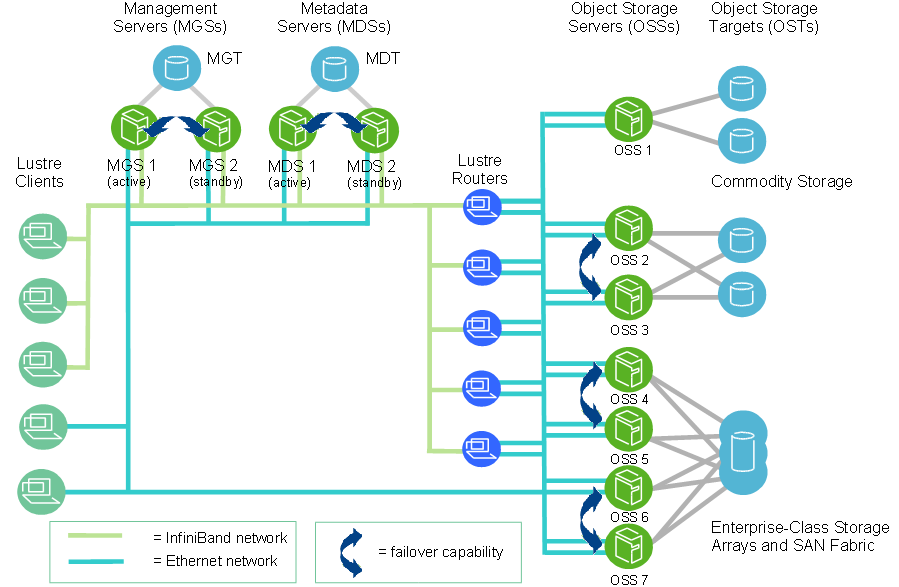
\includegraphics[width=1.0\linewidth]{scaled_cluster}}
\caption{Scaled Cluster}
\label{scaled_cluster}
\end{figure}

À grande échelle, un cluster de système de fichiers Lustre peut inclure des centaines de OSS et des milliers de clients, Figure \ref{scaled_cluster}, Plus d'un type de réseau peut être utilisé dans un cluster Lustre. Le stockage partagé entre OSS permet la fonction de basculement\textit{(failover)}.

\subsubsection{Stockage des données avec Lustre}

	Dans Lustre version 2.0, les identifiants de fichiers Lustre \textit{(File Identifier «FID») }ont été introduites pour remplacer les numéros d'inodes UNIX pour identifier des fichiers ou des objets. Un FID est un identificateur de 128 bits qui contient un numéro unique de 64 bits séquence, un 32-bit ID objet \textit{(Object Identifier «OID»)}, et un numéro de version 32 bits. Le numéro de séquence est unique parmi tous les objectifs Lustre dans un système de fichiers (OST et EMD). Ce changement a permis le soutien futur de plusieurs équipes multidisciplinaires (introduits dans Lustre version 2.3 du logiciel) et ZFS\footnote{http://fr.wikipedia.org/wiki/ZFS}(introduits dans Lustre logiciel version 2.4).\\

\begin{figure}[Donnes en Lustre]
\center{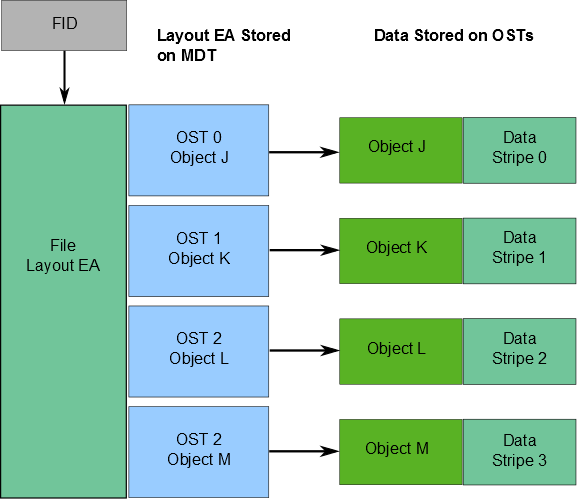
\includegraphics[width=0.5\linewidth]{dataenlustre}}
\caption{Disposition EA sur MDT pointant vers le fichier de données sur OST}
\label{dataenlustre}
\end{figure}

Informations sur l'endroit où les données de fichier se trouve sur le OST, est stockée comme un attribut étendu appelé disposition EA dans un objet MDT identifié par la FID pour le fichier(figure \ref{dataenlustre}). Si le fichier est un fichier de données (pas un répertoire ou un lien symbolique), l'objet MDT pointe de 1 à N OST objet(s) sur le(s) OST(s) qui contiennent les données de fichiers. Si le fichier MDT pointe à un objet, toutes les données de fichier sont stockées dans cet objet. Si le MDT pointe à plus d'un objet, les données du fichier sont réparties sur les objets à l'aide RAID 0, et chaque objet est stocké sur un OST différent.\\

Quand un client veut lire ou écrire dans un fichier, il récupère tout d'abord la mise en EA de l'objet MDT pour le fichier. Le client utilise ensuite ces informations pour effectuer des Entrées/Sorties sur le fichier, interagir directement avec les nœuds OSS où les objets sont stockés(Figure 4).

\begin{figure}[Client-FS]
\center{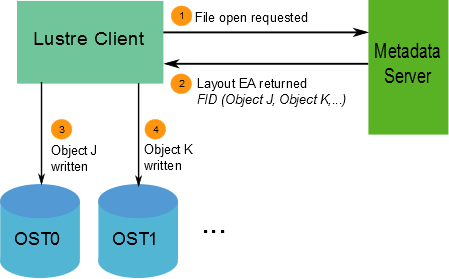
\includegraphics[width=0.6\linewidth]{file_write}}
\caption{Lustre client demandant des données}
\label{fig:identification}
\end{figure}

\newpage
\subsubsection{Lustre et l'entrelacement}

L'un des principaux facteurs menant à la haute performance des systèmes de fichiers Lustre est la capacité de répartir les données sur plusieurs OST dans un mode round-robin. Les utilisateurs peuvent éventuellement configurer pour chaque fichier le nombre de rayures, taille de bande, et OST qui sont utilisés. \\

L'entrelacement\textit{(Striping)} peut être utilisé pour améliorer les performances lorsque la bande passante globale à un fichier unique excède la bande passante d'un seul OST. La capacité de bande est également utile lorsque l'OST n'a pas assez d'espace pour contenir un fichier entier.

Le Stripping permet segments ou «morceaux» de données dans un fichier pour être stocké sur différents OST, dans le système de fichiers Lustre, une configuration RAID 0 est utilisée dans laquelle des données sont «striped» à travers un certain nombre d'objets. Le nombre d'objets dans un seul fichier est appelé \textit{stripe\_count}.

Chaque objet contient un bloc de données à partir du fichier. Lorsque le bloc de données en cours d'écriture à un objet particulier dépasse la \textit{stripe\_size}, le prochain bloc de données dans le fichier est stocké sur l'objet suivant.

Les valeurs par défaut pour \textit{stripe\_count} et \textit{stripe\_size} sont fixés pour le système de fichiers. La valeur par défaut pour \textit{stripe\_count} est une bande de fichier et la valeur par défaut pour \textit{stripe\_size} est 1Mo. L'utilisateur peut modifier ces valeurs sur une base par répertoire ou par fichier.

La taille maximale de fichier n'est pas limité par la taille d'une cible unique. Dans un système de fichiers Lustre, les fichiers peuvent être réparties sur plusieurs objets (jusqu'en 2000), et chaque objet peut être jusqu'à 16 To en taille avec ldiskfs\footnote{http://wiki.lustre.org/lid/ulfi/ulfi\_ldiskfs.html}. Cela conduit à une taille de fichier maximale de 31,25 pétaoctets. (Notez qu'un système de fichiers Lustre peut supporter des fichiers jusqu'à \begin{math}2^{64}\end{math} octets selon le stockage de sauvegarde utilisé par OST.)

\begin{figure}[Striping]
\center{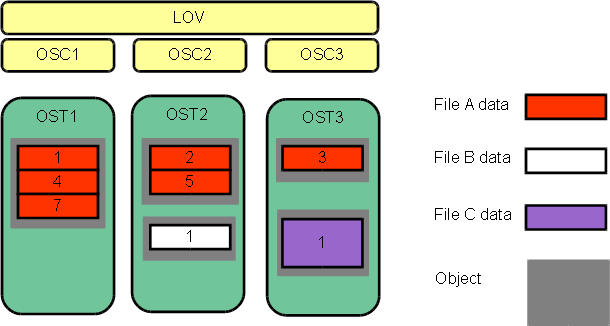
\includegraphics[width=0.6\linewidth]{file_striping}}
\caption{Striping}
\label{fig:identification}
\end{figure}


\newpage
\subsection{Installation}
\newpage
\subsubsection{Ubuntu-Lustre}
Parallèlement à la première tentative d'installation sur CentOS 6.5, en suivant la recommandation de notre tuteur, nous avons decidé de déployer les client Lustre dans une architecture virtualisée, mais en utilisant le système d'exploitation Ubuntu 13.10 cette fois.

Nous avons travaillé également avec KVM et l'outil graphique virt-manager pour créer une machine Virtuelle à laquelle nous avons attibué 7 cpus, 2 Go de mémoire vive et 20 Go de disque dur, cette machine etait destinée principalement à la compilation du noyau Linux version 3.13.6, qui donne la posibilité d'activer les frivers compatibles avec Lustre.

Le plan était compiler et installer le nouveau nouyau su cette machine et despuis les sources compiler les paquets nécesaires pour l'installation de Lustre sur chaque noeud, cloner la machine 2 fois, réduire ses resources pour les donner 2 cpus à chaqune et 1 Go de mémoire vive, deployer sur les machines clonées et la première machine les clients Lustre.

Nous avons commencé pour la compilation du noyau Linux v13.13.6, la dernière version «stable», nous sommes allés sur le site officiel\footnote{https://www.kernel.org/} pour télécharger les paquets sources.

On a obtenu le fichier «linux-3.13.6.tar.xz» dans notre machine virtuelle, pour extraire le contenu nous avons utilisé la commande:

\begin{verbatim}
	rsmrg@LUT:$tar -Jxvf linux-3.13.6.tar.xz
\end{verbatim}

Ensuite on a changé le répertoire pour nous déplacer vers celui que nous avons extrait du fichier, aussi on a installé les outils de compilation:

\begin{verbatim}
rsmrg@LUT:$cd linux-3.16.6 ; sudo apt-get install debconf-utils dpkg-dev
debhelper  build-essential kernel-package libncurses5-dev
\end{verbatim}

Nous avons copié la configuration du noyau précédant, après on a exécuté, make oldconfig pour répondre aux nouvelles questions de configurations du noyau:

\begin{verbatim}
rsmrg@LUT:$sudo cp /boot/config- 'uname -r' .config
rsmrg@LUT:$make oldconfig
\end{verbatim}

Pour activer les options Lustre on est allé au menu de configuration de noyau dans la partie «Staging drivers» (figure \ref{kernel}).

\begin{verbatim}
rsmrg@LUT:$make menuconfig
\end{verbatim}

\begin{figure}[Lustre Options]
\center{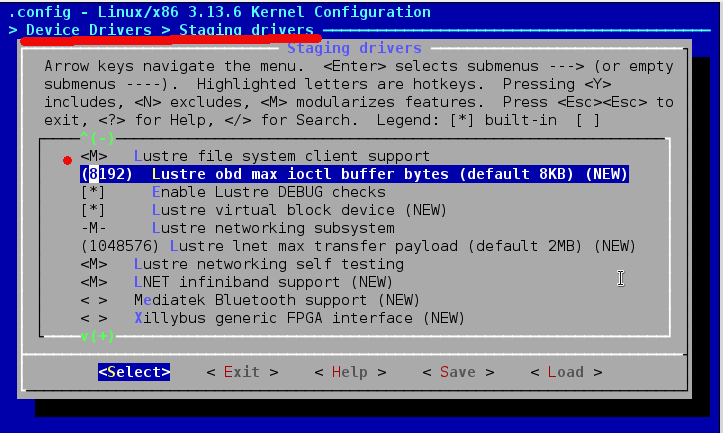
\includegraphics[width=0.8\linewidth]{kernel}}
\caption{Lustre Drivers}
\label{kernel}
\end{figure}

Après sauvegarder les manipulations réalisées, il fallait compiler le noyau en utilisant les 7 cpus et générer les paquets «.deb»:

\begin{verbatim}
rsmrg@LUT:$sudo make -j7 deb-pkg
\end{verbatim}

\begin{figure}[Compilation]
\center{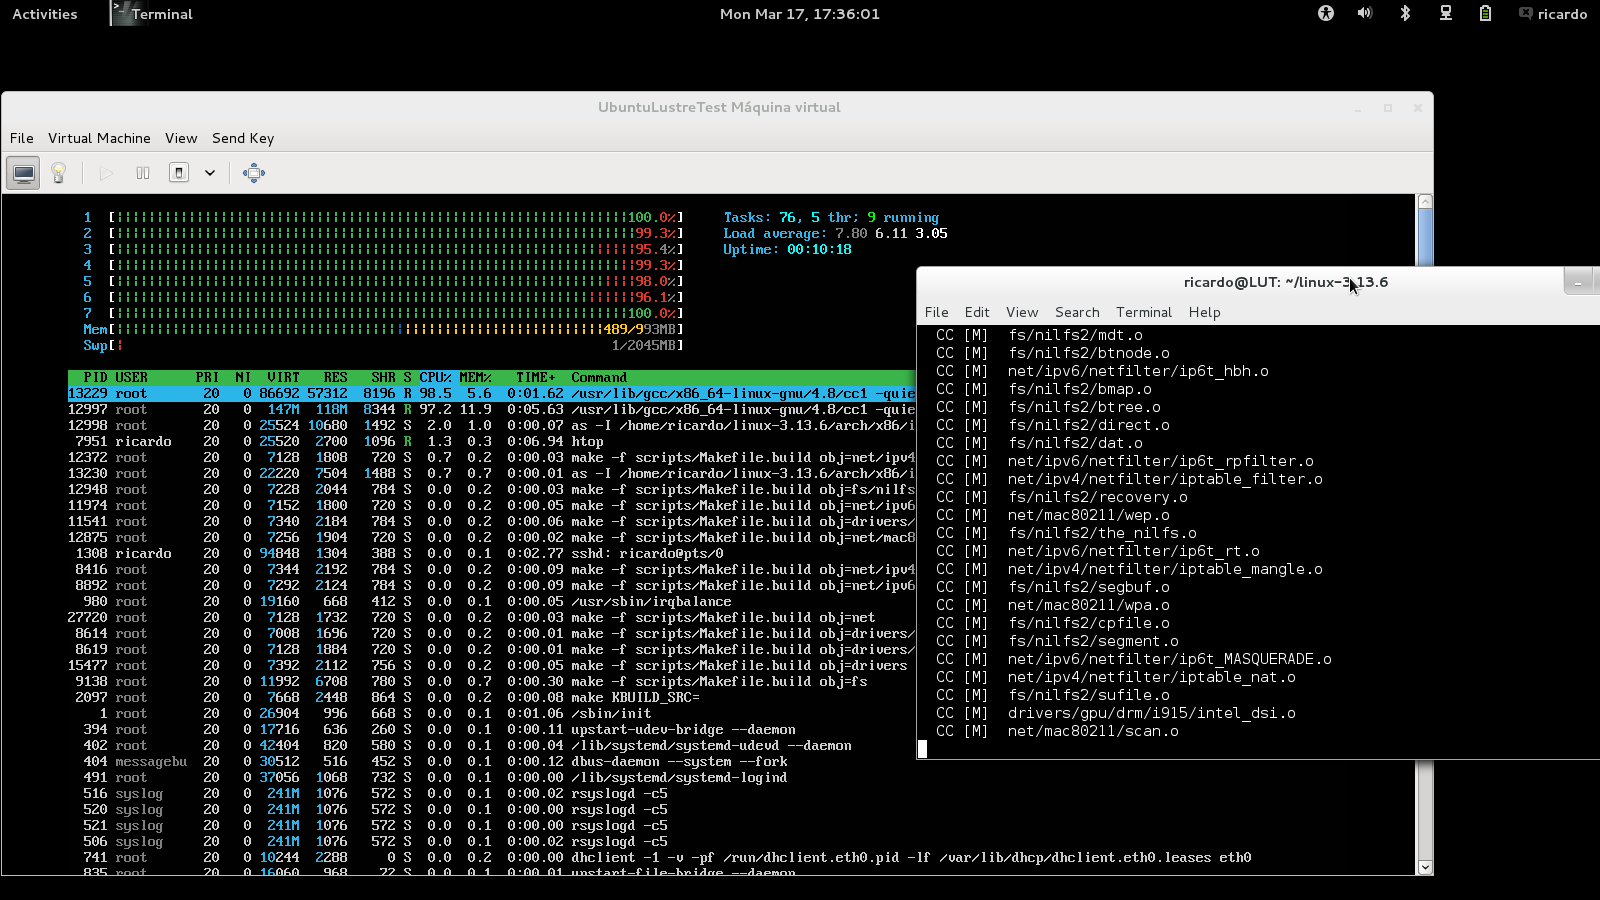
\includegraphics[width=0.8\linewidth]{compilation}}
\caption{Compilation Linux-13.13.6}
\label{kernel}
\end{figure}

Installation du nouveau kernel depuis les paquets généres:

\begin{verbatim}
rsmrg@LUT:$sudo dpkg -i ../*.deb
\end{verbatim}

Après la compilation du noyau de Linux on a essayé d'installer les paquets Lustre sur le système d'exploitation, mais sans succès, après avoir parlé avec le tuteur du projet, il a recommandé l'arrêt de travail avec Ubuntu pour  ne pas perdre plus de temps et de nous consacrer entièrement au déploimeent de Lustre avec logiciels plus anciens, mais supportés, comme c'est le cas du système d'exploitation CentOS 6.3.

\newpage
\subsection{QQLiéeàLustre}
\subsection{MásPerca}
\subsection{Lustre}
\subsection{Faru}
\section{Conclusion}

http://doc.ubuntu-fr.org/tutoriel/compiler\_linux 
http://wiki.lustre.org/manual/LustreManual18\_HTML/IntroductionToLustre.html
http://wiki.lustre.org/index.php/Debian\_Install
https://wiki.debian.org/Lustre
http://downloads.whamcloud.com/public/lustre/lustre-2.5.1/el6/client/RPMS/x86\_64/
http://ocubom.wordpress.com/2008/05/21/estructuras-basicas-de-latex/
http://en.wikipedia.org/wiki/Lustre\_(file\_system)

\end{document}
